\documentclass[conference]{IEEEtran}

% *** PACKAGES ***
\usepackage{cite}
\usepackage{amsmath,amssymb,amsfonts}
\usepackage{graphicx}
\usepackage{textcomp}
\usepackage{xcolor}
\usepackage{url}
% Added for figures
\usepackage{tikz}
\usetikzlibrary{arrows.meta,positioning,shapes,fit,calc}
\usepackage{pgfplots}
\pgfplotsset{compat=1.18}
\usepackage{tikz}

\begin{document}
	
	\title{Adaptive Container Scheduling for IoT-Based Real-Time Environmental Monitoring}
	
	\author{\IEEEauthorblockN{First Author, Second Author}
		\IEEEauthorblockA{Department of Computer Science \\
			XYZ University \\
			Email: first.author@xyz.edu, second.author@xyz.edu}}
	
	\maketitle
	\begin{abstract}
		The rapid proliferation of Internet of Things (IoT) devices has enabled real-time environmental monitoring across urban and rural settings. However, the dynamic workload and heterogeneous nature of fog and cloud infrastructures require efficient scheduling mechanisms to minimize latency, energy consumption, and cost. This paper proposes an \textit{Adaptive Container Scheduling Framework} that leverages fog and cloud resources in a hybrid manner. By dynamically migrating application containers based on workload intensity, network delay, and energy constraints, the proposed method achieves improved Quality of Service (QoS) for time-sensitive applications. The system is validated using \textit{iFogSim2} simulations, demonstrating significant improvements in latency, energy efficiency, and cloud cost over traditional static placement strategies.
	\end{abstract}
	
	\begin{IEEEkeywords}
		IoT, Fog Computing, Adaptive Scheduling, Container Orchestration, iFogSim2, Environmental Monitoring
	\end{IEEEkeywords}
	
	\section{Introduction}
	The Internet of Things (IoT) paradigm has transformed how environmental conditions are monitored and analyzed. Sensors deployed across cities can measure air quality, temperature, humidity, and pollutants to provide early warnings for public health and disaster management. However, these devices produce massive volumes of real-time data that must be processed with low latency. Traditional cloud-centric architectures introduce communication delays and high costs due to WAN transmission. Fog computing addresses these limitations by extending computational resources closer to the edge of the network. Nonetheless, static scheduling of tasks to fog or cloud nodes is inefficient under dynamic workloads.
	
	This work introduces an \textit{Adaptive Container Scheduling Framework} that dynamically places and migrates application modules between fog and cloud resources. The goal is to optimize latency, reduce energy consumption, and minimize cloud usage costs while preserving scalability.
	
	\section{Proposed Research Objectives}
	The following three objectives are designed to systematically advance the adaptive scheduling framework from a simulated concept to a field-tested, extensible, and industry-relevant system. Each objective addresses a key limitation of the initial study and moves the technology progressively closer to real-world applicability.
	
	\subsection{Integrate with Real-World Kubernetes Orchestration}
	Integrate with Real-World Kubernetes Orchestration
	This objective focuses on integrating our adaptive scheduling algorithm with Kubernetes, the de-facto industry standard for container orchestration. This involves developing a custom scheduler or operator that can implement our decision-making logic within a live Kubernetes cluster.
	Kubernetes integration is essential for practical adoption because it transforms the framework from a bespoke research tool into a component that can operate within the real-world IT ecosystems used by enterprises and service providers. Success here is the first step toward creating a deployable, production-grade solution.
	The expected outcome is a functional prototype where the adaptive scheduling logic can dynamically manage container placement and migration across a Kubernetes-managed cluster that spans both fog and cloud nodes.
	
	\subsection{Extend Framework to Support Multimedia Workloads}
	This objective aims to extend the framework's capabilities beyond the simple sensor data of the initial study to manage demanding multimedia workloads, specifically focusing on real-time video streams.
	This extension will demonstrate the framework's versatility and broaden its applicability to high-value domains. Unlike the low-data-rate environmental sensors, video streams have stringent high-bandwidth and low-latency requirements. Proving the framework's effectiveness for these workloads will validate its use in critical applications such as public safety monitoring, industrial automation, and smart city services.
	The expected outcome is a comprehensive performance analysis demonstrating the framework's ability to maintain Quality of Service (QoS) for real-time video stream processing, successfully balancing latency, energy, and cost under high-throughput conditions.
	
	
	\subsection{Validate Performance on a Physical IoT Testbed}
	This final objective is to deploy and validate the entire integrated system on a physical testbed composed of real IoT devices, fog nodes such as micro data centers or gateways, and cloud resources.
	This is the ultimate validation step. A physical testbed will expose the framework to real-world network conditions, hardware performance variance, and asynchronous events that cannot be perfectly modeled in simulation. This objective will provide definitive proof of the framework's efficacy and its tangible benefits in a live operational environment.
	The expected outcome is a comprehensive validation report that directly compares the performance metrics (latency, energy, cost) gathered from the physical testbed against the initial iFogSim2 simulation results, providing the first real-world proof of the adaptive scheduling framework's value.
	These well-defined objectives will be achieved through a structured and phased research plan detailed in the following section.
	\section{System Model and Problem Definition}
	\subsection{Architecture}
	The system comprises three layers:
	\begin{enumerate}
		\item \textbf{IoT Devices}: This layer consists of a variety of sensors deployed in the environment to measure critical parameters such as Air Quality Index (AQI), Temperature, Humidity, Pollution levels. Each sensor node is responsible for collecting real-time data and transmitting it to the nearest fog node for further processing. The deployment of heterogeneous sensors ensures comprehensive environmental monitoring.
		\item \textbf{Fog Layer:}
		The fog layer acts as an intermediate layer between IoT devices and the cloud. It comprises fog nodes (or edge gateways) that:
		\begin{itemize}
			\item Provide low-latency processing, enabling quick decision-making locally.
			\item Aggregate and pre-process sensor data before forwarding it to the cloud, reducing the communication overhead and network congestion.
			\item Support scalability by managing multiple sensor nodes and distributing computational tasks efficiently.
		\end{itemize}
		In the illustrated system, Fog Node 1 manages Sensor Node 1 (AQI) and Sensor Node 2 (Temperature), while Fog Node 2 manages Sensor Node 3 (Humidity) and Sensor Node 4 (Pollution).
		\item \textbf{Cloud Layer}: The cloud layer consists of centralized data centers that:
		\begin{itemize}
			\item Store large volumes of sensor data for long-term analysis.
			\item Offer scalable computational resources for advanced analytics, machine learning, and visualization.
			\item Ensure global accessibility, enabling stakeholders to access the processed data from anywhere.
		\end{itemize}
	\end{enumerate}
	
	\begin{figure}[htbp]
		\centering
		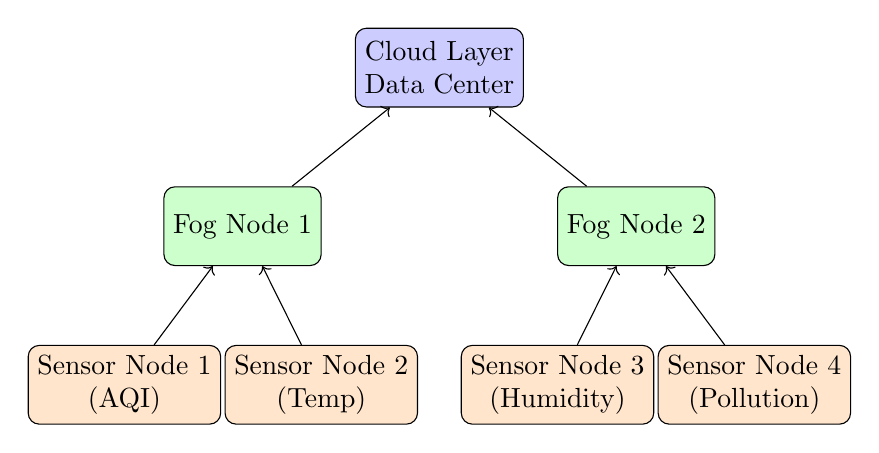
\begin{tikzpicture}[node distance=1cm, every node/.style={draw, rounded corners, align=center, minimum width=1cm, minimum height=1cm}]
			
			% Cloud
			\node[fill=blue!20] (cloud) {Cloud Layer\\Data Center};
			
			% Fog
			\node[fill=green!20, below=of cloud, xshift=-2.5cm] (fog1) {Fog Node 1};
			\node[fill=green!20, below=of cloud, xshift=2.5cm] (fog2) {Fog Node 2};
			
			% Sensors
			\node[fill=orange!20, below=of fog1, xshift=-1.5cm] (sensor1) {Sensor Node 1\\(AQI)};
			\node[fill=orange!20, below=of fog1, xshift=1cm] (sensor2) {Sensor Node 2\\(Temp)};
			\node[fill=orange!20, below=of fog2, xshift=-1cm] (sensor3) {Sensor Node 3\\(Humidity)};
			\node[fill=orange!20, below=of fog2, xshift=1.5cm] (sensor4) {Sensor Node 4\\(Pollution)};
			
			% Connections
			\draw[->] (sensor1) -- (fog1);
			\draw[->] (sensor2) -- (fog1);
			\draw[->] (sensor3) -- (fog2);
			\draw[->] (sensor4) -- (fog2);
			
			\draw[->] (fog1) -- (cloud);
			\draw[->] (fog2) -- (cloud);
			
		\end{tikzpicture}
		\caption{System architecture showing IoT sensors, fog nodes, and cloud data center.}
		\label{fig:architecture}
	\end{figure}
	\subsection{Communication Model}
	The communication flow follows a hierarchical structure:
	\begin{enumerate}
		\item \textbf{Sensor-to-Fog Communication:} IoT sensors periodically transmit data to the associated fog node via short-range wireless communication (e.g., Wi-Fi, Zigbee, or LoRa).
		\item  \textbf{Fog-to-Cloud Communication:} Processed or aggregated data is forwarded from fog nodes to the cloud layer using high-bandwidth connections. This step ensures that only essential data is sent to the cloud, optimizing network usage.
	\end{enumerate}
	The primary objective of the system is to \textbf{monitor environmental conditions in real-time and enable rapid response.} The key challenges addressed by this architecture include:
	\begin{enumerate}
		\item \textbf{Low-latency Data Processing:} Some applications, such as pollution alerts or emergency responses, require immediate action, which the fog layer facilitates.
		\item \textbf{Scalability:} The system must handle a growing number of sensor nodes without overwhelming the network or cloud resources.
		\item \textbf{Efficient Data Management:} By processing data at the fog layer, redundant transmissions are minimized, reducing storage requirements and energy consumption.
		\item \textbf{Data Reliability:} Hierarchical data aggregation ensures robustness against individual sensor failures.
	\end{enumerate}
	\subsection{Advantages of the Three-Layer Architecture}
	\begin{enumerate}
		\item \textbf{Reduced Latency:} Local processing at fog nodes ensures that time-sensitive data is acted upon immediately.
		\item \textbf{Optimized Bandwidth:} Only relevant data is sent to the cloud, decreasing unnecessary data traffic.
		\item \textbf{Enhanced Scalability:} New sensors can be easily integrated by connecting to existing or new fog nodes.
		\item \textbf{Centralized Analytics:} The cloud layer enables complex analytics, trend detection, and predictive modeling.
	\end{enumerate}
	
		
\end{document}
	